\documentclass{article}
\usepackage[paperwidth=14.25in,paperheight=7.35in,margin=0.06in]{geometry}
\usepackage{amsmath}
\usepackage{tikz}
\usetikzlibrary{arrows.meta,positioning,calc}
\pagestyle{empty}
\pgfdeclarelayer{panelbg}
\pgfdeclarelayer{backline}
\pgfsetlayers{panelbg,backline,main}

\begin{document}
\noindent
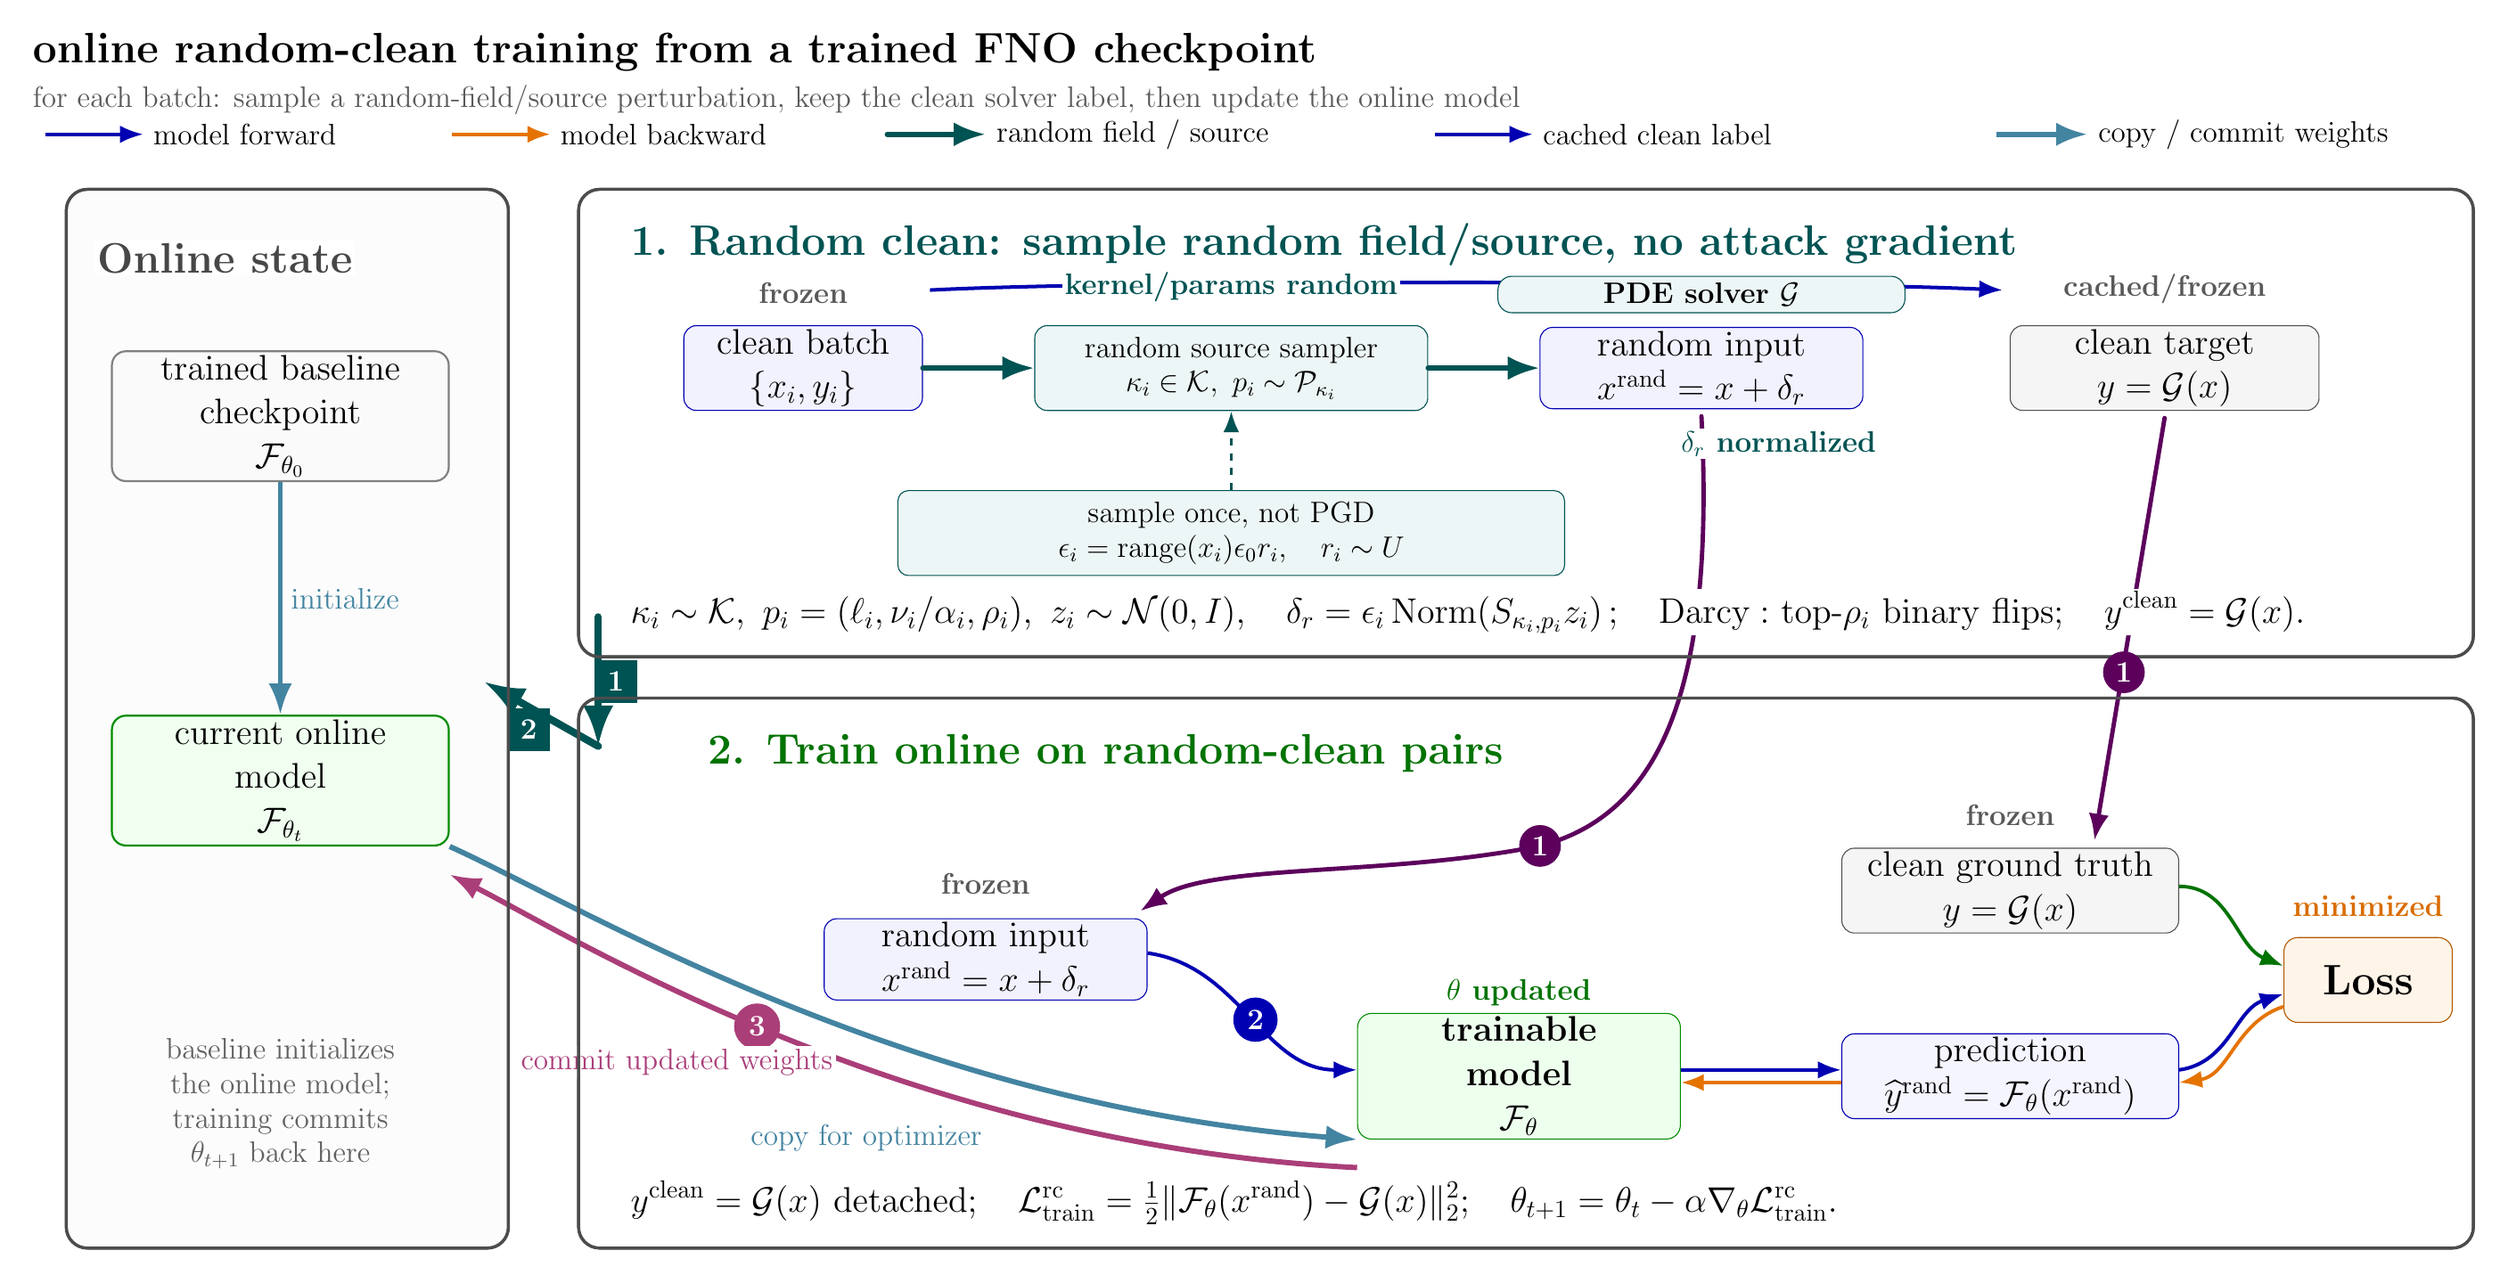
\begin{tikzpicture}[
  x=1mm,y=0.98mm,
  >=Latex,
  font=\sffamily,
  panel/.style={draw=black!65, rounded corners=3mm, line width=1.05pt, fill=white},
  state/.style={draw=black!50, rounded corners=2mm, line width=0.8pt, fill=black!2, minimum width=46mm, minimum height=12.1mm, align=center, font=\Large, inner ysep=1.5pt},
  input/.style={draw=blue!70!black, rounded corners=1.8mm, fill=blue!5, minimum width=38mm, minimum height=11mm, align=center, font=\Large, inner ysep=1.4pt},
  sampler/.style={draw=teal!65!black, rounded corners=1.8mm, fill=teal!7, minimum width=56mm, minimum height=12.1mm, align=center, font=\large, inner ysep=1.3pt},
  solver/.style={draw=teal!65!black, rounded corners=2mm, fill=teal!7, minimum width=42mm, minimum height=12.1mm, align=center, font=\Large\bfseries, inner ysep=1.4pt},
  model/.style={draw=green!55!black, rounded corners=2mm, fill=green!7, minimum width=46mm, minimum height=13.2mm, align=center, font=\Large\bfseries, inner ysep=1.4pt},
  labelbox/.style={draw=gray!65!black, rounded corners=1.8mm, fill=gray!8, minimum width=48mm, minimum height=11mm, align=center, font=\Large, inner ysep=1.4pt},
  outbox/.style={draw=blue!70!black, rounded corners=1.8mm, fill=blue!4, minimum width=48mm, minimum height=11mm, align=center, font=\Large, inner ysep=1.4pt},
  loss/.style={draw=orange!70!black, rounded corners=2mm, fill=orange!9, minimum width=24mm, minimum height=12.1mm, align=center, font=\LARGE\bfseries, inner ysep=1.3pt},
  epsbox/.style={draw=teal!65!black, rounded corners=1.5mm, fill=teal!7, minimum width=95mm, minimum height=12.1mm, align=center, font=\large, inner ysep=1.2pt},
  label/.style={font=\LARGE\bfseries, anchor=west, fill=white, inner sep=1pt},
  formula/.style={font=\Large, anchor=south west, align=left, fill=white, inner sep=1pt},
  note/.style={font=\large, text=black!65, align=left},
  smallnote/.style={font=\large\bfseries, text=black!65, align=center, anchor=south},
  action/.style={font=\large\bfseries, align=center, anchor=south},
  fwd/.style={->, draw=blue!70!black, line width=1.45pt},
  cleanlabel/.style={->, draw=blue!70!black, line width=1.45pt, solid},
  bmodel/.style={->, draw=orange!90!black, line width=1.4pt},
  solverline/.style={->, draw=green!45!black, line width=1.4pt},
  handoffone/.style={->, draw=violet!72!black, line width=1.75pt, line cap=round},
  randline/.style={->, draw=teal!65!black, line width=2.2pt, line cap=round},
  handoff/.style={->, draw=teal!70!black, line width=2.05pt, line cap=round},
  cacheline/.style={->, draw=gray!62!black, line width=1.25pt, dashed},
  copyarr/.style={->, draw=cyan!60!black, line width=2.15pt},
  copytwo/.style={->, draw=cyan!60!black, line width=2.15pt},
  copythree/.style={->, draw=magenta!65!black, line width=2.15pt},
  macrocycle/.style={->, draw=teal!65!black, line width=3.0pt, line cap=round},
  numone/.style={circle, draw=violet!72!black, fill=violet!72!black, text=white, inner sep=1.1pt, outer sep=0pt, minimum size=5.8mm, font=\large\bfseries},
  numtwo/.style={circle, draw=blue!70!black, fill=blue!70!black, text=white, inner sep=1.1pt, minimum size=5.8mm, font=\large\bfseries},
  numthree/.style={circle, draw=magenta!65!black, fill=magenta!65!black, text=white, inner sep=1.1pt, minimum size=5.8mm, font=\large\bfseries},
  macronum/.style={draw=teal!65!black, fill=teal!65!black, text=white, inner sep=0pt, minimum width=5.9mm, minimum height=5.9mm, font=\large\bfseries}
]

% Title and compact legend
\node[font=\LARGE\bfseries, anchor=west] at (5,176)
  {online random-clean training from a trained FNO checkpoint};
\node[note, anchor=west] at (5,169)
  {for each batch: sample a random-field/source perturbation, keep the clean solver label, then update the online model};

\draw[fwd] (8,164) -- ++(14,0) node[right, black, font=\large] {model forward};
\draw[bmodel] (66,164) -- ++(14,0) node[right, black, font=\large] {model backward};
\draw[randline] (128,164) -- ++(14,0) node[right, black, font=\large] {random field / source};
\draw[cleanlabel] (206,164) -- ++(14,0) node[right, black, font=\large] {cached clean label};
\draw[copyarr] (286,164) -- ++(13,0) node[right, black, font=\large] {copy / commit weights};

% Left online-state column.
\begin{pgfonlayer}{panelbg}
  \draw[panel, fill=black!1] (11,2) rectangle (74,156);
\end{pgfonlayer}
\node[label, text=black!72] at (15,146) {Online state};
\node[state, minimum width=48mm] (baseline) at (41.5,123)
  {trained baseline\\checkpoint\\$\mathcal F_{\theta_0}$};
\node[state, minimum width=48mm, draw=green!55!black, fill=green!6] (current) at (41.5,70)
  {current online\\model\\$\mathcal F_{\theta_t}$};
\node[font=\large, text=black!62, align=center] at (41.5,23)
  {baseline initializes\\the online model;\\training commits\\$\theta_{t+1}$ back here};
\draw[copyarr] (baseline) -- node[right, font=\large, text=cyan!60!black] {initialize} (current);

% ================= Random clean generation panel =================
\begin{scope}[shift={(84,88)}]
  \begin{pgfonlayer}{panelbg}
    \draw[panel] (0,0) rectangle (270,68);
  \end{pgfonlayer}
  \node[label, text=teal!65!black] at (7,60) {1. Random clean: sample random field/source, no attack gradient};

  \node[input, minimum width=34mm] (clean) at (32,42)
    {clean batch\\$\{x_i,y_i\}$};
  \node[sampler] (sampler) at (93,42)
    {random source sampler\\$\kappa_i\in\mathcal K,\ p_i\sim\mathcal P_{\kappa_i}$};
  \node[input, minimum width=46mm] (xrandgen) at (160,42)
    {random input\\$x^{\rm rand}=x+\delta_r$};
  \node[labelbox, minimum width=44mm] (ycleangen) at (226,42)
    {clean target\\$y=\mathcal G(x)$};
  \node[epsbox] (epsnote) at (93,18)
    {sample once, not PGD\\$\epsilon_i={\rm range}(x_i)\epsilon_0 r_i,\quad r_i\sim U$};

  \node[smallnote] at (32,50.1) {frozen};
  \node[smallnote, text=teal!65!black, fill=white, inner sep=1pt] at (93,51.2) {kernel/params random};
  \node[font=\large\bfseries, text=teal!65!black, align=center, fill=white, inner sep=1pt]
    at (171,31) {$\delta_r$ normalized};
  \node[smallnote] at (226,50.1) {cached/frozen};

  \draw[randline] (clean) -- (sampler);
  \draw[randline] (sampler) -- (xrandgen);
  \begin{pgfonlayer}{panelbg}
  \draw[cleanlabel] ([xshift=1mm,yshift=5mm]clean.north east)
    .. controls (78,54.8) and (170,54.8) ..
    ([xshift=-1mm,yshift=5mm]ycleangen.north west);
  \end{pgfonlayer}
  \node[solver, minimum width=58mm, minimum height=5.2mm, font=\large\bfseries, inner ysep=0pt]
    at (160,52.7) {PDE solver $\mathcal G$};
  \draw[cacheline, draw=teal!65!black] (epsnote.north) -- (sampler.south);

  \node[formula] at (7,3.0)
    {$\displaystyle \kappa_i\sim\mathcal K,\ p_i=(\ell_i,\nu_i/\alpha_i,\rho_i),\ z_i\sim\mathcal N(0,I),\quad
      \delta_r=\epsilon_i\,{\rm Norm}\!\left(S_{\kappa_i,p_i}z_i\right);\quad
      {\rm Darcy:}\ {\rm top}\text{-}\rho_i\ {\rm binary\ flips};\quad
      y^{\rm clean}=\mathcal G(x).$};
\end{scope}

% ================= Training panel =================
\begin{scope}[shift={(84,2)}]
  \begin{pgfonlayer}{panelbg}
    \draw[panel] (0,0) rectangle (270,80);
  \end{pgfonlayer}
  \fill[white] (16,67) rectangle (145,78);
  \node[label, text=green!45!black] at (18,72) {2. Train online on random-clean pairs};

  \node[input, minimum width=46mm] (xrandtrain) at (58,42)
    {random input\\$x^{\rm rand}=x+\delta_r$};
  \node[labelbox] (ycleantrain) at (204,52)
    {clean ground truth\\$y=\mathcal G(x)$};
  \node[model] (tmodel) at (134,25)
    {trainable\\model\\$\mathcal F_\theta$};
  \node[outbox] (ypred) at (204,25)
    {prediction\\$\widehat y^{\rm rand}=\mathcal F_\theta(x^{\rm rand})$};
  \node[loss] (tloss) at (255,39) {Loss};

  \node[smallnote] at (58,50.2) {frozen};
  \node[smallnote] at (204,60.2) {frozen};
  \node[smallnote, text=green!45!black] at (134,34.0) {$\theta$ updated};
  \node[action, text=orange!85!black] at (255,47.0) {minimized};

  \draw[solverline] ([yshift=0.6mm]ycleantrain.east) to[out=0,in=158] ([yshift=2mm]tloss.west);
  \draw[fwd] ([yshift=0.9mm]xrandtrain.east)
    to[out=-8,in=180]
    node[pos=0.52, numtwo] {2}
    ([yshift=0.9mm]tmodel.west);
  \draw[fwd] ([yshift=0.9mm]tmodel.east) -- ([yshift=0.9mm]ypred.west);
  \draw[fwd] ([yshift=0.9mm]ypred.east) to[out=8,in=198] ([yshift=-2.0mm]tloss.west);
  \draw[bmodel] ([yshift=-3.8mm]tloss.west) to[out=198,in=8] ([yshift=-0.9mm]ypred.east);
  \draw[bmodel] ([yshift=-0.9mm]ypred.west) -- ([yshift=-0.9mm]tmodel.east);

  \node[formula] at (7,3.0)
    {$\displaystyle y^{\rm clean}=\mathcal G(x)\ {\rm detached};\quad
      \mathcal L_{\rm train}^{\rm rc}=\tfrac12\|\mathcal F_\theta(x^{\rm rand})-\mathcal G(x)\|_2^2;\quad
      \theta_{t+1}=\theta_t-\alpha\nabla_\theta\mathcal L_{\rm train}^{\rm rc}.$};
\end{scope}

% Random input and clean label are handed from the generation panel into training.
\begin{pgfonlayer}{backline}
\draw[handoffone] ([yshift=-1.0mm]xrandgen.south)
  .. controls (246,83) and (238,65.0) ..
  (221,60.5) coordinate (xrandcleanone)
  .. controls (199,56.0) and (174,58.0) ..
  ([xshift=22mm,yshift=1.0mm]xrandtrain.north);
\end{pgfonlayer}
\node[numone] at (xrandcleanone) {1};

% Cached clean target is passed into the training panel as a solid clean-label flow.
\begin{pgfonlayer}{backline}
\draw[handoffone] ([yshift=-1.0mm]ycleangen.south)
  -- coordinate[pos=0.58] (ycleancleanone)
  ([xshift=12mm,yshift=1.0mm]ycleantrain.north);
\end{pgfonlayer}

% Small panel-level cycle: keep the main figure's second and third edges.
\draw[macrocycle] (86.8,93.8) -- (86.8,75.0);
\node[macronum] at (89.3,84.4) {1};
\draw[macrocycle] (86.8,75.0) -- (70.5,84.4);
\node[macronum] at (76.9,77.4) {2};

% Copy current model to optimizer, then commit update.
\begin{pgfonlayer}{backline}
\draw[copytwo] (current.south east)
  .. controls (84,52) and (130,23) ..
  (tmodel.south west);
\draw[copythree] ([yshift=-4mm]tmodel.south west)
  .. controls (130,17) and (82,48) ..
  node[pos=0.52, numthree] {3}
  ([yshift=-4mm]current.south east);
\end{pgfonlayer}
\node[font=\large, text=cyan!60!black, fill=white, inner sep=1.5pt]
  at (125,18) {copy for optimizer};
\node[font=\large, text=magenta!65!black, fill=white, inner sep=1.5pt]
  at (98,29) {commit updated weights};

% Redraw the online-state and stage borders on the foreground so vertical edges match top/bottom.
\draw[draw=black!70, rounded corners=3mm, line width=1.25pt, line join=round] (11,2) rectangle (74,156);
\draw[draw=black!70, line width=1.25pt, line cap=round] (11,5) -- (11,153);
\draw[draw=black!70, line width=1.25pt, line cap=round] (74,5) -- (74,153);
\draw[draw=black!70, rounded corners=3mm, line width=1.25pt] (84,88) rectangle (354,156);
\draw[draw=black!70, rounded corners=3mm, line width=1.25pt] (84,2) rectangle (354,82);

% Keep this handoff marker above all borders and labels.
\node[numone] at ([yshift=-1.3mm]ycleancleanone) {1};

\end{tikzpicture}
\end{document}
